\documentclass[12pt,a4paper]{article}
\usepackage[utf8]{inputenc}
\usepackage{graphicx}  
\usepackage{amsmath}
\usepackage{amsfonts}
\usepackage{amssymb}
\usepackage{gensymb}  % degree symbols
\author{Richard Decal}
\title{%
  Solving Cartpole Using Reinforcement Learning and Policy Gradients \\
  \large Machine Learning Engineer Nanodegree\\
  Capstone Project}
\usepackage[style=numeric,sorting=none,backend=bibtex]{biblatex}
\addbibresource{references.bib}
%\bibliographystyle{unsrt}

\begin{document}

\maketitle


\section{Definition}
%_(approx. 1-2 pages)_

\subsection*{Project Overview}
%In this section, look to provide a high-level overview of the project in layman’s terms. Questions to ask yourself when writing this section:
%- _Has an overview of the project been provided, such as the problem domain, project origin, and related datasets or input data?_
%- _Has enough background information been given so that an uninformed reader would understand the problem domain and following problem statement?_

Reinforcement learners are a class of algorithms which learn to perform a task by sampling legal actions and recieving feedback from its environment. The algorithm uses the feedback to optimize its behavior to maximize future rewards. These algorithms can amazingly become proficient at a given task-- outperforming humans in some domains-- without ever being given explicit directions, rules, explanations, or any domain knowledge whatsoever. Given enough time to test various strategies, a good reinforcement learning algorithm will converge to the optimal decision policy.

In this work, I will use reinforcement learning to solve ``CartPole", a classic control problem with a binary choice at each timestep. This problem was first solved using neural network-like algorithms in 1983.\cite{og_cartpole} Reinforcement learning is capable of learning this task due to its relatively small state and output spaces.\cite{deep_pg}\cite{ddpg_blog}

\subsection*{Problem Statement}
%In this section, you will want to clearly define the problem that you are trying to solve, including the strategy (outline of tasks) you will use to achieve the desired solution. You should also thoroughly discuss what the intended solution will be for this problem. Questions to ask yourself when writing this section:
%- _Is the problem statement clearly defined? Will the reader understand what you are expecting to solve?_
%- _Have you thoroughly discussed how you will attempt to solve the problem?_
%- _Is an anticipated solution clearly defined? Will the reader understand what results you are looking for?_

\begin{figure}[htbp]
\begin{center}
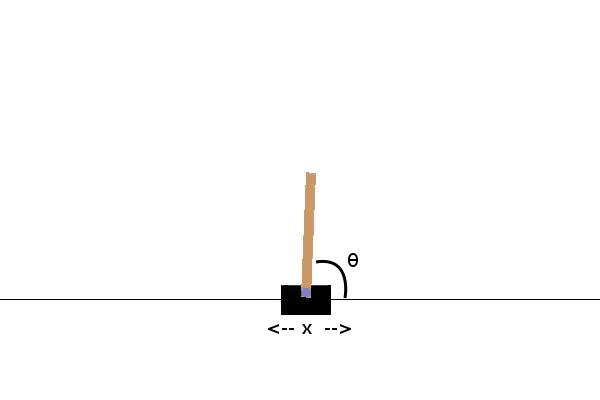
\includegraphics[scale=0.66]{cartpole.jpg}
\caption{Screenshot of the CartPole-v0 game. The $x$ position and angle $\theta$ are labeled.}
\label{cartpole}
\end{center}
\end{figure}

``CartPole" is a simple 2D game which simulates an upright pole connected by a hinge to a cart.\cite{cartpole} The cart moves freely on a frictionless surface (Figure \ref{cartpole}). Each trial is initiated with the cart at the center of the environment and the pole upright. At each timestep, the agent has to choose between pushing the cart to left or to the right.  For each timestep in a trial, the game returns a return signal of +1 point. The trial ends if any of these conditions are met:




\begin{itemize}
 \item  the pole tilts 15$\degree$ away from vertical
 \item the cart has moved out of bounds
 \item the time limit (200 timesteps) is reached
 \end{itemize}
 
My goal for this project is to train an algorithm which can maintain the pole upright and within bounds for all 200 timesteps in as few trials as possible. To do this, I will use neural networks to compute output probabilities of the appropriate actionat each timestep. Then, I will modify the reward vector from the environment such that the algorithm can discriminate between good and bad actions (otherwise, all the rewards will always be +1). I will do this using Bellman's Equation (discussed later). Then, I will use the rewards to scale a loss function, solve the gradient of the loss function with respect to the network parameters, and use that to update the network parameters. 

\subsection*{Metrics}
%In this section, you will need to clearly define the metrics or calculations you will use to measure performance of a model or result in your project. These calculations and metrics should be justified based on the characteristics of the problem and problem domain. Questions to ask yourself when writing this section:
%- _Are the metrics you’ve chosen to measure the performance of your models clearly discussed and defined?_
%- _Have you provided reasonable justification for the metrics chosen based on the problem and solution?_

The most salient metric is episode length, as the game is defined as solved when the algorithm can stay ``alive" for the entire 200 timestep limit.

The second metric will be histograms of the pole's angle $\theta$. We expect these to collapse to a single peak near zero (corresponding to an upright pole) in an optimally behaving policy.

Initially, I created a bonus system to reward states with the pole upright and the cart close to the center of the track, with the rational that these are states which are least likely to lead to failure. However, I disabled those because they amounted to injecting prior domain knowledge into the reward system. I thought it would be more interesting to create an algorithm which learned good states from a completely naive starting point. In addition, a short-lived trajectory could get relatively high bonus points simply due to the fact that it spent a relatively high fraction of the time in states which reward bonuses.

Finally, one might expect to examine the discounted rewards which the agent uses to improve its own performance. However, as we will see later, these have been mean subtracted and scaled down to unit variance. The effect is that, no matter which actions are taken, late timesteps are always punished, and early timesteps are always rewarded. As we will see, this reward structure is sufficient to encourage a policy to solve the game. However, the reward history and its summary statistics (mean, variance, etc.) has limited use for comparing models after the fact.


\section{Analysis}
%_(approx. 2-4 pages)_
%
\subsection*{Data Exploration}
%In this section, you will be expected to analyze the data you are using for the problem. This data can either be in the form of a dataset (or datasets), input data (or input files), or even an environment. The type of data should be thoroughly described and, if possible, have basic statistics and information presented (such as discussion of input features or defining characteristics about the input or environment). Any abnormalities or interesting qualities about the data that may need to be addressed have been identified (such as features that need to be transformed or the possibility of outliers). Questions to ask yourself when writing this section:
%- _If a dataset is present for this problem, have you thoroughly discussed certain features about the dataset? Has a data sample been provided to the reader?_
%- _If a dataset is present for this problem, are statistics about the dataset calculated and reported? Have any relevant results from this calculation been discussed?_
%- _If a dataset is **not** present for this problem, has discussion been made about the input space or input data for your problem?_
%- _Are there any abnormalities or characteristics about the input space or dataset that need to be addressed? (categorical variables, missing values, outliers, etc.)_

For this task, my learner will be totally naive and will have no previous data to inform the policy. The game environment has a convenient open-source wrapper provided by OpenAI which allows us to step through trials.\cite{cartpole} At each timestep, the game provides the agent the current environment state as well as the reward for the action taken at the previous timestep.  The sensory input is the cart's position $x$, the cart's velocity $\dot x$, the pole's angle $\theta$ (measured in radians), and its rate of change $\dot\theta$ (see Figure \ref{cartpole}).\cite{state_def} 

Given the state and the chosen action, the agent is given immediate feedback from the game in the form of a reward. These (state, action, reward) pairs are crucial for the reinforcement algorithm to improve its policy from its experiences (discussed in the project design section).

I initially thought of reducing the state space to simply the $x$ position and $\theta$. However, the problem with that is the agent has no way of knowing from a single frame whether the speed at which the pole and cart are moving. If the system is rapidly moving in one direction, it is important for the agent to oppose that movement to cancel it out, or otherwise the CartPole will be have too much momentum to prevent it reaching an absorbing state.


%\subsection*{Exploratory Visualization}
%In this section, you will need to provide some form of visualization that summarizes or extracts a relevant characteristic or feature about the data. The visualization should adequately support the data being used. Discuss why this visualization was chosen and how it is relevant. Questions to ask yourself when writing this section:
%- _Have you visualized a relevant characteristic or feature about the dataset or input data?_
%- _Is the visualization thoroughly analyzed and discussed?_
%- _If a plot is provided, are the axes, title, and datum clearly defined?_
%
\subsection*{Algorithms and Techniques}
%In this section, you will need to discuss the algorithms and techniques you intend to use for solving the problem. You should justify the use of each one based on the characteristics of the problem and the problem domain. Questions to ask yourself when writing this section:
%- _Are the algorithms you will use, including any default variables/parameters in the project clearly defined?_
%- _Are the techniques to be used thoroughly discussed and justified?_
%- _Is it made clear how the input data or datasets will be handled by the algorithms and techniques chosen?_

I tried various reinforcement algorithms in the course of the project. Initially, I attempted to use an actor critic network. The name refers to the two neural networks which comprise the algorithm: a critic network and an actor network. The critic takes a series of (state, action) pairs and outputs a reward vector, wheras the actor takes states as an input and computes the probability it should take different actions. The actor's optimizer tries to maximze the rewards it will recieve from the critic. 

I also tried a policy gradient algorithm without a critic network. In place of the critic network, I passed the environemental rewards through Bellman's Equation to get discounted rewards (discussion in the ``implementation" section). These discounted rewards were then used to calculate the loss for each particular action, and an Adam optimizer was used to minimze the loss.

The actor-only algorithm is much simpler due to the fact that it is comprised of only one neural network instead of two. The actor network takes states and outputs action probabilities. The network is comprised of one or more fully connected layers, which are then passed through a sigmoid activation function.

Specifics about implementation of these algorithms are discussed in ``Implementation" section.


\subsection*{Benchmark}
%In this section, you will need to provide a clearly defined benchmark result or threshold for comparing across performances obtained by your solution. The reasoning behind the benchmark (in the case where it is not an established result) should be discussed. Questions to ask yourself when writing this section:
%- _Has some result or value been provided that acts as a benchmark for measuring performance?_
%- _Is it clear how this result or value was obtained (whether by data or by hypothesis)?_
To establish a baseline, I created two simple models to compare my policy gradient algorithm. The first is a random actor, which takes a random action at each timestep. The second is a ``contrarian'' actor. The contrarian actor simply looks at which direction the pole is tilting, and always pushes the pole towards the upright position.

The random policy had an average episode length of approximately 20 timesteps, and the contrarian model had an average episode length of approximatly 45 timesteps (details in the results section). 

\section{Methodology}
%_(approx. 3-5 pages)_
%
\subsection*{Data Preprocessing}
%In this section, all of your preprocessing steps will need to be clearly documented, if any were necessary. From the previous section, any of the abnormalities or characteristics that you identified about the dataset will be addressed and corrected here. Questions to ask yourself when writing this section:
%- _If the algorithms chosen require preprocessing steps like feature selection or feature transformations, have they been properly documented?_
%- _Based on the **Data Exploration** section, if there were abnormalities or characteristics that needed to be addressed, have they been properly corrected?_
%- _If no preprocessing is needed, has it been made clear why?_
We did not preprocess any data before starting training as we did not have a starting dataset prior to the reinforcement learning.


\subsection*{Implementation}
%In this section, the process for which metrics, algorithms, and techniques that you implemented for the given data will need to be clearly documented. It should be abundantly clear how the implementation was carried out, and discussion should be made regarding any complications that occurred during this process. Questions to ask yourself when writing this section:
%- _Is it made clear how the algorithms and techniques were implemented with the given datasets or input data?_
%- _Were there any complications with the original metrics or techniques that required changing prior to acquiring a solution?_
%- _Was there any part of the coding process (e.g., writing complicated functions) that should be documented?_

I began trying to solve CartPole using an actor-critic model. However, after a few days of work I could not make any progress getting it to learn, no matter which parameters and architectures I tried. In order to make headway on my project, I switched to policy gradients without a critic network, which has less than half the number of parameters and complexity.

Once I switched to the policy gradient algorithm, I tested it with various architectures and hyperparameters. I tested up to four fully connected layers. I tried between 10 and 200 neurons per layer, using dropout layers, and adding biases to the lairs. I also tested various functions: tanh, sigmoid, and softmax. A graph of my final model is shown in Figure \ref{actor_net}.


Instead of having a neural network representing the reward function as in a deep Q network, I used the rewards provided by the environement. However, if all actions are equally labeled as being worth +1 rewards, the algorithm has no way of descriminating between good actions and bad actions. I achieved this using the classic Bellman's Equation (Equation \ref{bellman}):

\begin{equation}\label{bellman}
D(a_i) = R(a_i) + \sum_{n=i+1}^{\infty}{ \gamma R(a_n)} 
\end{equation}

The $R(a)$ term represents the reward for a particular action, which was always +1. The second term $\gamma \sum_{n=i+1}^{\infty}{R(a_n)}$ is the sum of all future rewards, where each reward is diminished by $\gamma$, a scaling or discount factor. Discounted rewards are a way of projecting consequences of future states to actions taken in the past.

The discounted rewards were further processed by subtracting the mean and dividing by the standard deviation. Subtracting the mean promotes actions with higher-than-expected rewards, and penalizes ones that give below-average rewards. Dividing by the standard deviation made training more stable, since the rewards had much lower variance. The combination of these transformations reduce the computation needed by the optimizer as well and prevent floating arithmetic errors.

This works fairly well, but the training is very volatile because the discount reward always rewards early actions and penalizes late actions, regardless of which actions were actually chosen. The rational is that trajectories which last longer are associated with discount reward vectors which strongly encourage the early actions, which will have accumulated a large discounted reward. As we will see in the conclusion, this has a deleterious effect at the later stages of training.

To further reduce variance, I tried two different batching techniques. One is to save all the (state,action,reward) pairs into a replay buffer, and after a certain amount of trials solve the discounted reward across all the different trajectories in the mini batch. The advantage of this is that when we subtract the mean and standard deviation it will be of our entire batch. Thus, each indiviual action are scored against a larger pool of actions and the model can better discriminate between good and bad actions.

Similarly, I tried using batched gradients. During each episode in the batch, we compute the gradient of the loss with respect to our parameters and add it to the running gradient sum vector. We continue to add each computed gradient into the batch gradient. This smooths out the volatility in the gradients because while sometimes the gradients are positive, and sometimes negative, they will all sum together and approximate the central tendency of the batch.



\begin{figure}[htbp]
\begin{center}
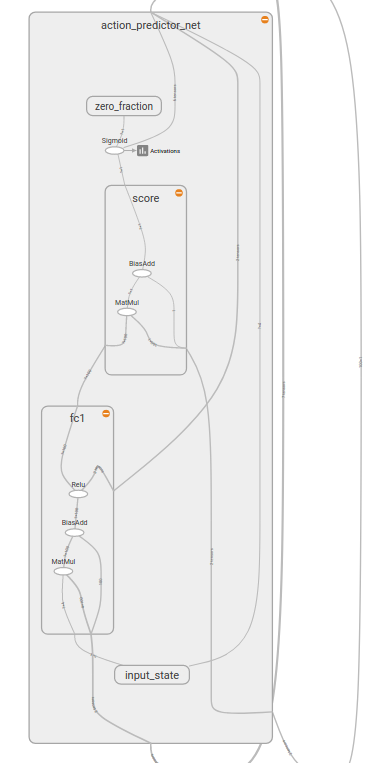
\includegraphics[scale=0.66]{actor_net.png}
\caption{Graph of my finalized actor network architecture. Input state is our observed state for that timestep. fc1 is a fully-connected layer with a ReLu activation. Score is a second fully connected layer. Finally, the scores are given to a sigmoid activation layer which outputs a single value between 0 and 1. This is the probability of choosing ``push right" action at that timestep.}
\label{actor_net}
\end{center}
\end{figure}


I had a very hard time getting to the point where any of my models would train. At first, my intuition was to take the brute force approach and add more nodes and layers to my model and let it train for more iterations. The rational was that a more complicated model has more degrees of freedom and could thus represent a more complex function which could solve my problem. At one point, I let the actor-critic model train overnight on my GPU with over 200,000 episodes, but it never converged to a solution.

After that, I reduced the complexity of my algorithm by removing the critic network. I tried various architectures: more layers, fewer layers, adding biases, different activation functions, different loss and optimization functions, using dropout layers, different learning rates. Nothing seemed to work.

Finally, I found a policy gradient implementation which solved CartPole on Github.\cite{gh_pg} I took it and progressively changed my hyperparameters and network architecture to match the functioning example. It still did not train. The last two differences in my model architecture were the ones which were impeding training. One was my weights initialization, which was using truncated normals. As soon as I changed it to an xavier intialization, my model started to train successfully. The other was the use of biases in one of the hidden layers. I was able to reliably reproduce the problem simply by switching the weights initialization back and forth between xavier and truncated normals, or by adding biases to the particular fully connected layer.



\subsection*{Refinement}
%In this section, you will need to discuss the process of improvement you made upon the algorithms and techniques you used in your implementation. For example, adjusting parameters for certain models to acquire improved solutions would fall under the refinement category. Your initial and final solutions should be reported, as well as any significant intermediate results as necessary. Questions to ask yourself when writing this section:
%- _Has an initial solution been found and clearly reported?_
%- _Is the process of improvement clearly documented, such as what techniques were used?_
%- _Are intermediate and final solutions clearly reported as the process is improved?_



With my model finally training, I started optimizing the parameters and architecture. The original implementation used only 10 neurons per layer and it took 2000 episodes to solve CartPole. I created a series of nested for loops to do a large parameter sweep of possible models to rule out certain architectures by examining their properties in Tensorboard. In this way, I tested over 100 model architectures. Table \ref{table:param_space} shows the parameters tested.

\begin{table}

\begin{center}
\begin{tabular}{ c  c p{5cm}}
  Parameter & Values or Ranges tested & Notes  \\
  \hline
  Number of units per layer & 10 to 200 &  \\
  Batch size & 1 to 20 &  Number of episodes to run before optimizing.\\
  Learning rate& 1e-1 to 1e-6 & \\
  Use dropout layer & True/False & Used 50\% dropout rate. \\
  Use second hidden layer & True/False & \\
  Weight initialization & Truncated normal or xavier & Using truncated normal broke training.\\
  Use bias & True/False & Where to bias the outputs of our hidden fully connected layers.\\

\end{tabular}
\caption{Model parameters tested.}
\label{table:param_space}
\end{center}

\end{table}

Predictably, I found that the following things slowed down training time: using dropout layers, gradient batches, extra layers, and lower learning rates. As I iteratively reduced the scope of my parameter space scope, my models trained faster and faster, and I could reduce the number of episodes per model. Finally, I found a model which could reliably get a perfect score in less than 30 episodes, and sometimes as low as 13 episodes (discussed in the Model Evaluation section).



\section{Results}
%_(approx. 2-3 pages)_
%
\subsection*{Model Evaluation and Validation}
%In this section, the final model and any supporting qualities should be evaluated in detail. It should be clear how the final model was derived and why this model was chosen. In addition, some type of analysis should be used to validate the robustness of this model and its solution, such as manipulating the input data or environment to see how the model’s solution is affected (this is called sensitivity analysis). Questions to ask yourself when writing this section:
%- _Is the final model reasonable and aligning with solution expectations? Are the final parameters of the model appropriate?_
%- _Has the final model been tested with various inputs to evaluate whether the model generalizes well to unseen data?_
%- _Is the model robust enough for the problem? Do small perturbations (changes) in training data or the input space greatly affect the results?_
%- _Can results found from the model be trusted?_

\subsubsection*{Random Policy}

The random policy had a high variance in performance, with episodes lasting between 10 and 40 timesteps (Figure \ref{rand_ep_length}).  The average episode length is approximately 20 timesteps. Likewise, the distribution of thetas has a high spread (Figure \ref{rand_thetas}). The distributions do not change over time, which is expected since this policy does not learn. The clustering of values near zero is expected because the game is instantiated with the pole upright, and because episodes tend to last a very short time.

\begin{figure}[htbp]
\begin{center}
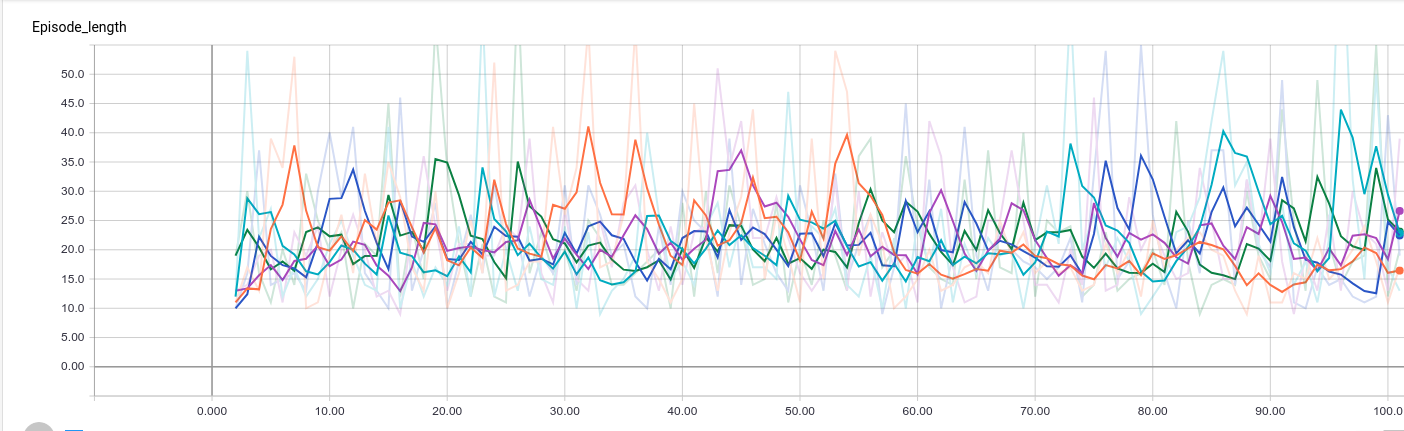
\includegraphics[width=\linewidth]{rand_ep_length.png}
\caption{Average timesteps per episode for random policy. The x-axis represents the episode number and the y-axis is the number of timesteps before the episode ended. The different colors represent different trials. As expected, the agent does not improve over time.}
\label{rand_ep_length}
\end{center}
\end{figure}

\begin{figure}[htbp]
\begin{center}
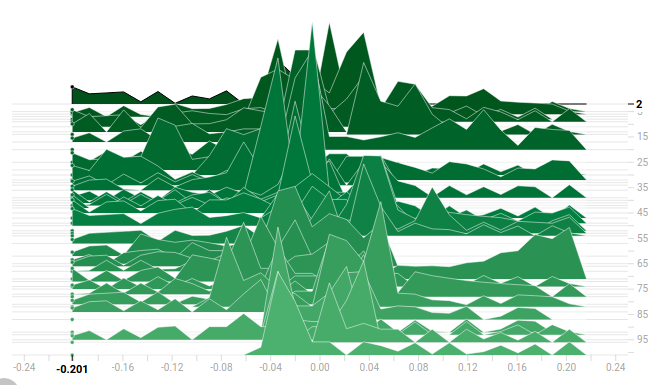
\includegraphics[width=\linewidth]{rand_thetas.png}
\caption{Histogram of thetas for random policy. The x-axis represents the angle in radians, with 0 being vertical. The height represents the frequency which that angle was observed. The depth represents the episode number, with histograms near the top being early episodes and the ones at the forefront being the final episodes.}
\label{rand_thetas}
\end{center}
\end{figure}

\subsubsection*{Contrarian Policy}

The average episode length is approximately 45 timesteps, which is more than twice as good as taking random actions (Figure \ref{pg_episodes}). As expected, the agent does not improve over time.  Qualitatively, the tails of the theta distributions (Figure \ref{contrarian_thetas}) are significantly smaller than the random agent, indicating that the pole spends more time balanced near the center. The distributions do not change over time, which is expected since this policy does not learn. 

\begin{figure}[htbp]
\begin{center}
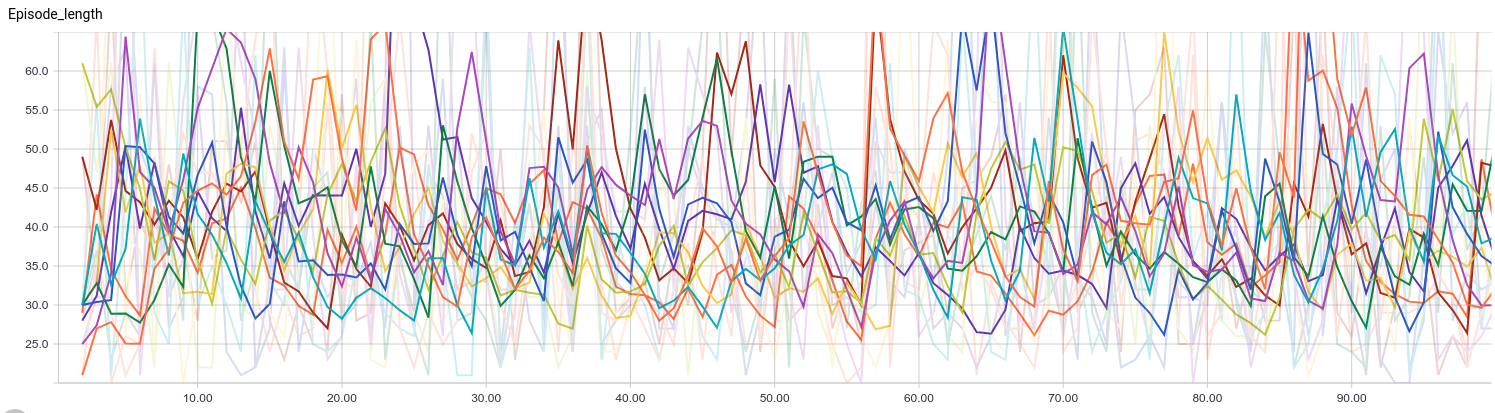
\includegraphics[width=\linewidth]{contrarian_lengths.png}
\caption{Average timesteps per episode for the contrarian policy. The different colors represent different trials. The x-axis represents the episode number and the y-axis is the number of timesteps before the episode ended. }
\label{contrarian_lengths}
\end{center}
\end{figure}

\begin{figure}[htbp]
\begin{center}
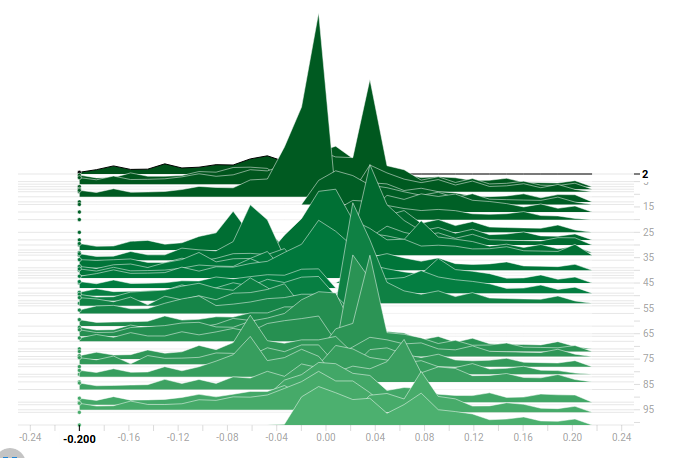
\includegraphics[width=\linewidth]{contrarian_thetas.png}
\caption{Histogram of thetas for contrarian policy. The x-axis represents the angle in radians, with 0 being vertical. The height represents the frequency which that angle was observed. The depth represents the episode number, with histograms near the top being early episodes and the ones at the forefront being the final episodes.}
\label{contrarian_thetas}
\end{center}
\end{figure}

\subsubsection*{Policy Gradient}

The final optimized model usually plays a perfect game within 35 episodes (Figure \ref{pg_episodes}), which is substantially better than the random actor's performance. Sometimes, it plays a perfect game in as little as 13 episodes. On the other hand, 

However, while these find the game quickly, the combination of a high learning rate and a noisy reward signal results in very high variance and inconsitent results. Sometimes it takes over 100 episodes to play a perfect game using the same exact model parameters (see the dark blue trace). Occaisionally, the model even catastrophically collapses (discussed in conclusion).

Letting the optimizer continue after we have solved the game inevitably causes the agent to stop playing optimally. This is because the reward function penalizes things near the end, even if doing well. This is advantageous for fast training, but bad once have solved the game.

\begin{figure}[htbp]
\begin{center}
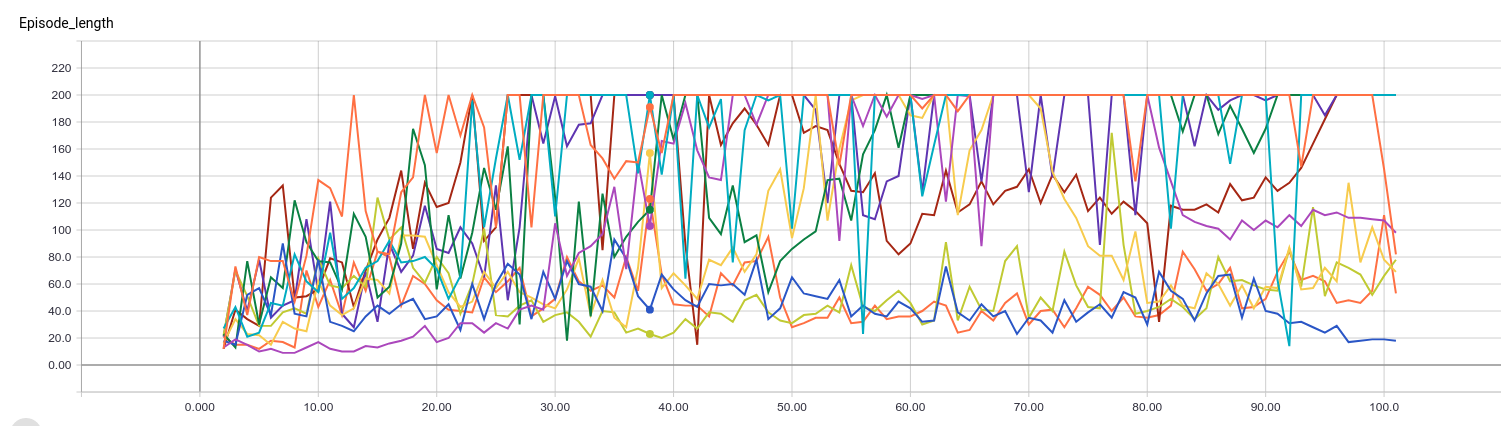
\includegraphics[width=\linewidth]{pg_episodes.png}
\caption{Episode lengths for the final policy gradient model.  The x-axis represents the episode number and the y-axis is the number of timesteps before the episode ended. The different colors represent different trials.  }
\label{pg_episodes}
\end{center}
\end{figure}

\begin{figure}[htbp]
\begin{center}
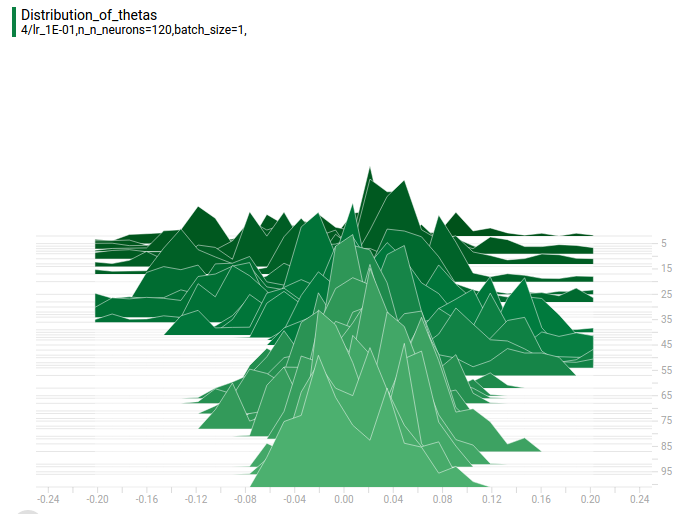
\includegraphics[width=\linewidth]{pg_thetas.png}
\caption{Histogram of thetas for policy gradient. The x-axis represents the angle in radians, with 0 being vertical. The height represents the frequency which that angle was observed. The depth represents the episode number, with histograms near the top being early episodes and the ones at the forefront being the final episodes.}
\label{pg_thetas}
\end{center}
\end{figure}

\subsection*{Justification}
%In this section, your model’s final solution and its results should be compared to the benchmark you established earlier in the project using some type of statistical analysis. You should also justify whether these results and the solution are significant enough to have solved the problem posed in the project. Questions to ask yourself when writing this section:
%- _Are the final results found stronger than the benchmark result reported earlier?_
%- _Have you thoroughly analyzed and discussed the final solution?_
%- _Is the final solution significant enough to have solved the problem?_
The policy gradient is capable of learning to solving the game, whereas the random and contrarian agents do not perform well and do not improve their performance over time. The random policy rarely exceeds an episode length of 50, the contrarian policy rarely exceeds an episode length of 70, wheras the final policy gradient model can repeatedly reach a perfect episode length of 200. The policy gradient is clearly the superior model.

\section{Conclusion}
%_(approx. 1-2 pages)_
%
\subsection*{Free-Form Visualization}
%In this section, you will need to provide some form of visualization that emphasizes an important quality about the project. It is much more free-form, but should reasonably support a significant result or characteristic about the problem that you want to discuss. Questions to ask yourself when writing this section:
%- _Have you visualized a relevant or important quality about the problem, dataset, input data, or results?_
%- _Is the visualization thoroughly analyzed and discussed?_
%- _If a plot is provided, are the axes, title, and datum clearly defined?_
%



I selected a trial where the model failed to train. I looked at the distribution of activations and weights over time, and it was clear that something was wrong (Figure \ref{pg_stuck}). The outputs tended to be zeros or ones, indicating that the model always picked a single direction to push the cart in. I examined the weights for the units in the actor network, and saw that early in the training the weights catastrophically converged to zeros, becoming impossible to update through matrix multiplication. These ``dead models" happened roughly 10\% of the time, which is to be expected with our aggressive learning rate and lack of batching.
 

\begin{figure}[htbp]
\begin{center}
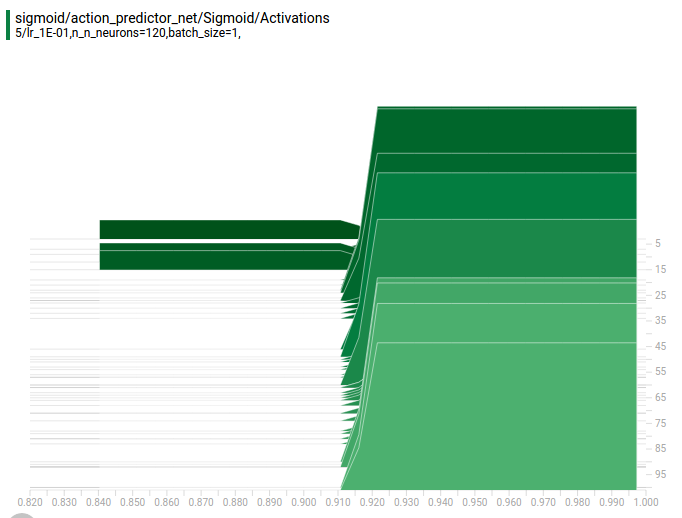
\includegraphics[width=\linewidth]{pg_stuck.png}
\caption{Activation over time of the actor network for each episode in the policy gradient. Note, unlike the figures above, these are not histograms-- the values are in chronologically ordered. The x-axis represents the run-time of a given episode, the height represents the output value of the sigmoid function. The depth represents the episode number, with histograms near the top being early episodes and the ones at the forefront being the final episodes. Values of 0 are a correspond to a high probability of pushing the cart to the left, and values near 1 correspond to a high probability of pushing the cart to the right.}
\label{pg_stuck}
\end{center}
\end{figure}

\subsection*{Reflection}
%In this section, you will summarize the entire end-to-end problem solution and discuss one or two particular aspects of the project you found interesting or difficult. You are expected to reflect on the project as a whole to show that you have a firm understanding of the entire process employed in your work. Questions to ask yourself when writing this section:
%- _Have you thoroughly summarized the entire process you used for this project?_
%- _Were there any interesting aspects of the project?_
%- _Were there any difficult aspects of the project?_
%- _Does the final model and solution fit your expectations for the problem, and should it be used in a general setting to solve these types of problems?_
If I had to give myself advice, it would be to start with a simple network architecture and expand the model from there. I started with an actor-critic model, which was too ambitious and much harder to debug when there were multiple bugs compounding each other.

I wish I would have started using Tensorboard summaries sooner. They proved invaluable in troubleshooting, once I figured out how to produce the summaries correctly.

\subsection*{Improvement}
%In this section, you will need to provide discussion as to how one aspect of the implementation you designed could be improved. As an example, consider ways your implementation can be made more general, and what would need to be modified. You do not need to make this improvement, but the potential solutions resulting from these changes are considered and compared/contrasted to your current solution. Questions to ask yourself when writing this section:
%- _Are there further improvements that could be made on the algorithms or techniques you used in this project?_
%- _Were there algorithms or techniques you researched that you did not know how to implement, but would consider using if you knew how?_
%- _If you used your final solution as the new benchmark, do you think an even better solution exists?_

In terms of converging in fewer episodes, I doubt there are many more gains than I can make while not imposing biases using prior knowledge. If adding prior knowledge into the model was allowed, I would add a bonus for low theta values to encourage the gradients to reward actions which lead to those states.

To prevent the problem with the network untraining themselves, I would stop updating the network parameters once the game is reliably beating the game. If I wanted a more stable algorithm, I would stop mean subtracting the discounted rewards, which always punishes actions taken at the end of an episode, even if they were good actions. I would also make the learning rate decay after each optimization step, as large optimization steps can push the model out of the global minimum. Finally, I would reduce the learning rate and start using batches again. These all cause the model training to slow down, but guarantees a more reliable algorithm overall.


%
%**Before submitting, ask yourself. . .**
%
%- Does the project report you’ve written follow a well-organized structure similar to that of the project template?
%- Is each section (particularly **Analysis** and **Methodology**) written in a clear, concise and specific fashion? Are there any ambiguous terms or phrases that need clarification?
%- Would the intended audience of your project be able to understand your analysis, methods, and results?
%- Have you properly proof-read your project report to assure there are minimal grammatical and spelling mistakes?
%- Are all the resources used for this project correctly cited and referenced?
%- Is the code that implements your solution easily readable and properly commented?
%- Does the code execute without error and produce results similar to those reported?

\printbibliography

\end{document}